\clearpage
\thispagestyle{empty}
~\clearpage
%\graphicspath{{Figures_chapter-4/}}
%\chapter{New Finite Difference Approach Involving Interfacial Points For Solving Immersed Interface Problems And Its Application to Stokes Flows}
%\chapter{New Finite Difference Approach Involving Interfacial Points For Solving Arbitrary Shaped Interface Problems in Cartesian Coordinates}
%\chapter{Interfacial Points Based Finite Difference Scheme For Solving Interface Problems in Cartesian Coordinates}
\chapter{Network Topology and Scanning Techniques}
\label{chap4}
\section{Reconnaissance Deception System}
The RDS configuration discussed by \cite{7971943} proposes that a different virtual network view can be assigned to every host or to specific hosts. Hence, the defense approach will be independent of the source of malicious scanners. It provides a clear separation between virtual views, that are only visible to the assigned malicious hosts, and the remaining underlying network.

Zero-day attacks, manual infection of hosts inside organizational networks are serious threats which can cause significant damage and are difficult to detect. Our system considers adversaries that are present inside our network and have at least one host infected with their malware.

The set of information collected by attackers during reconnaissance or probing phase is identified. We studied different configurations and possibilities for the generation of virtual network topologies using SDN in which nodes with critical information can be placed strategically to delay their detection by attackers.

To evaluate the deception strategy for the RDS configuration defined in \cite{7971943}, we implemented a simulated network prototype of RDS, based on Software Defined Networking(SDN), to simulate complete virtual network topologies including its physical network characteristics.

In our deception systems, honeypots are an essential component for trapping hackers. Honeypots are used during the simulation of virtual network views. Our virtual networks use honeypots as decoy system  to detect malicious attackers and identify adversaries.

We aim to deceive malicious attackers and network discovery techniques by showing a virtual view of the network which hides its true underlying network and its vulnerabilities that can be used by adversaries to exploit these weak points in the network. The simulation of a virtual network invalidates the information set of the adversaries about the network and achieves the goal of delaying the rate of identifying vulnerable hosts by a significant time. This additional time can be used to identify a malicious attacker and isolate it from the network.

\FloatBarrier
\begin{figure}[!htbp]
\centering
  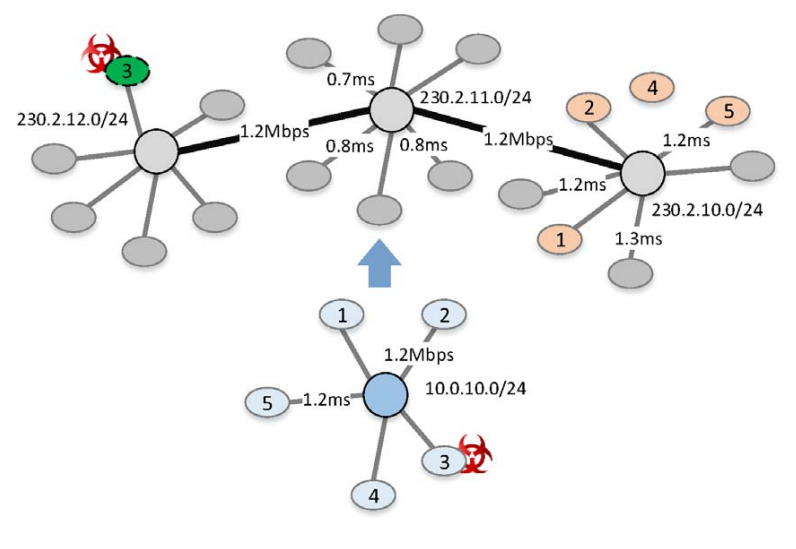
\includegraphics[scale=0.65]{Chap4/achle.png}
  \caption{Deceiving adversaries by projecting a virtual network where critical resources are at the periphery of network.}\label{fig:figure13}
\end{figure} 


\FloatBarrier
\begin{figure}[!htbp]
\centering
  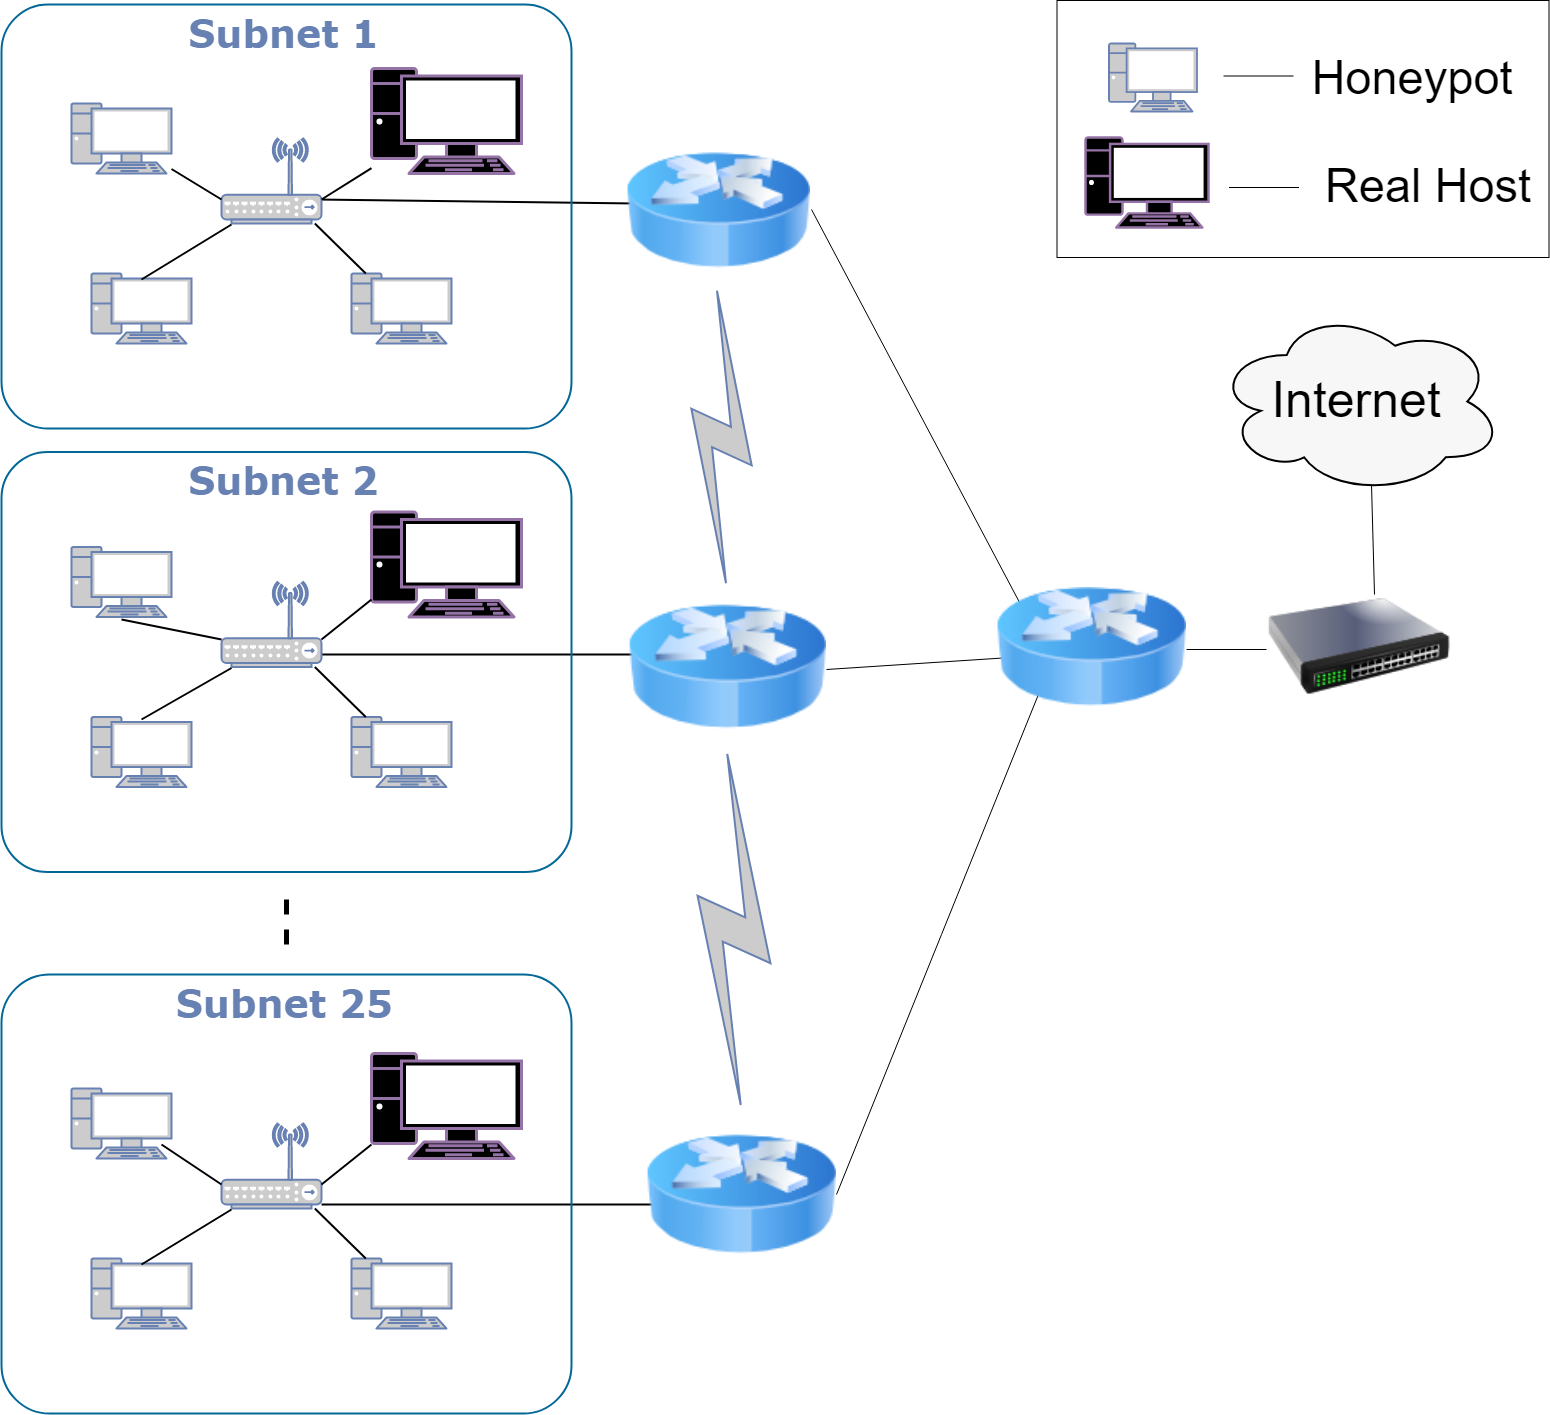
\includegraphics[scale=0.2]{Chap4/RDSConfig.png}
  \caption{RDS configuration}\label{fig:figure14}
\end{figure} 


\section{Non-RDS}
Non RDS configuration consists of a network of hosts connected to a single central host. Hence the entire network can be probed from the central host. The hosts in the Non-RDS configuration can easily be exploited if the central host in the network is compromised.Non RDS configuration contains the real information carrying hosts in proportion with a larger number of honeypots hosts to deceive the
intruders. The network view described in the previous chapters were Non-RDS.
   \FloatBarrier
    \begin{figure}[!htbp]
    \centering
      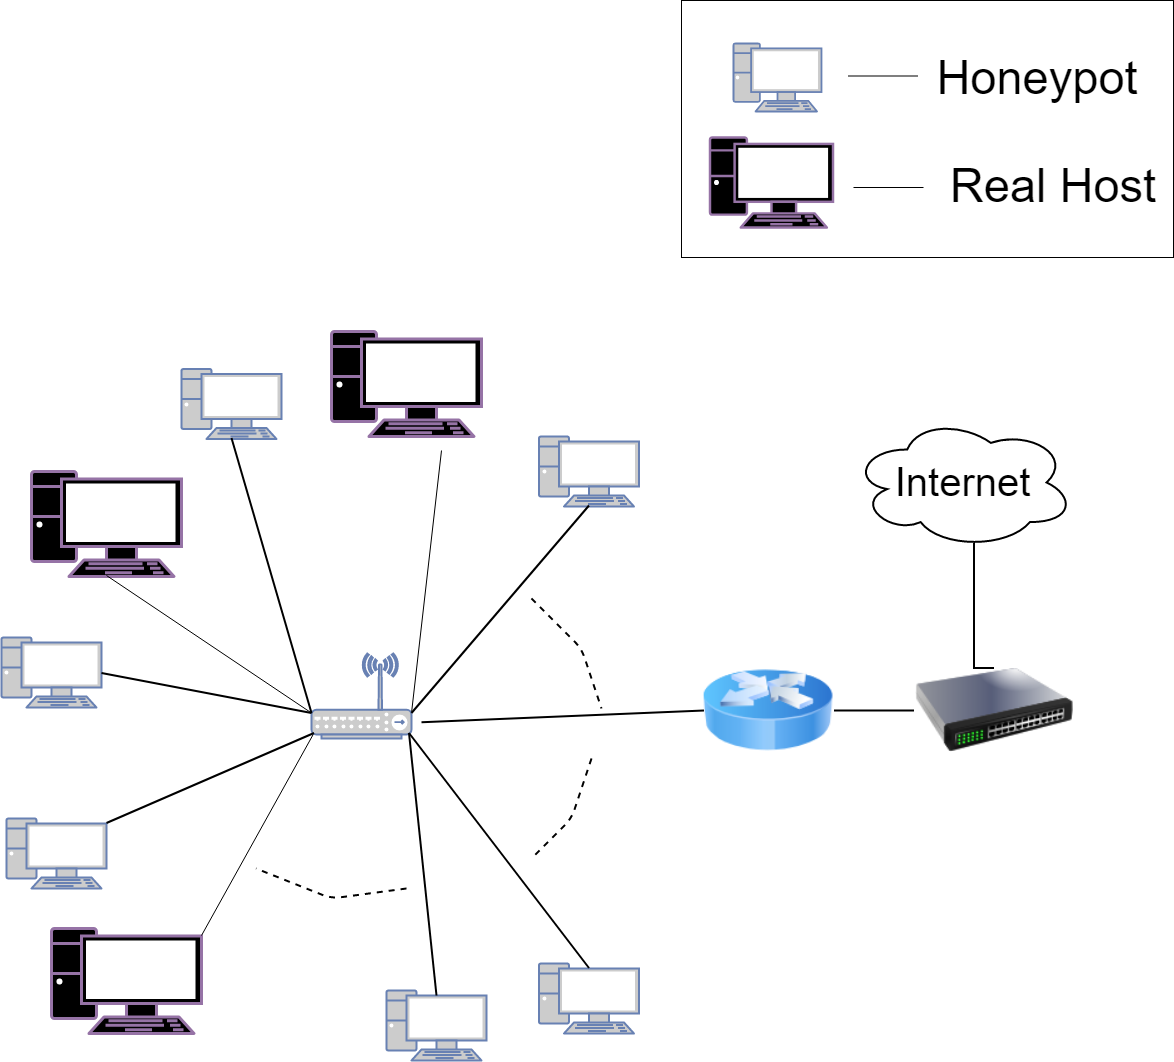
\includegraphics[scale=0.2]{Chap4/Non-RDS.png}
      \caption{Non-RDS Configuration}\label{fig:figure15}
    \end{figure} 


\section{Mixed Configuration}
Mixed Configuration is a topology midway between the two configurations discussed above. It has the characterstics of both the above network views. A few real systems are divided within the subnet part. The rest of the real systems are in the Non-RDS part of the configuration.
    \FloatBarrier
    \begin{figure}[!htbp]
    \centering
      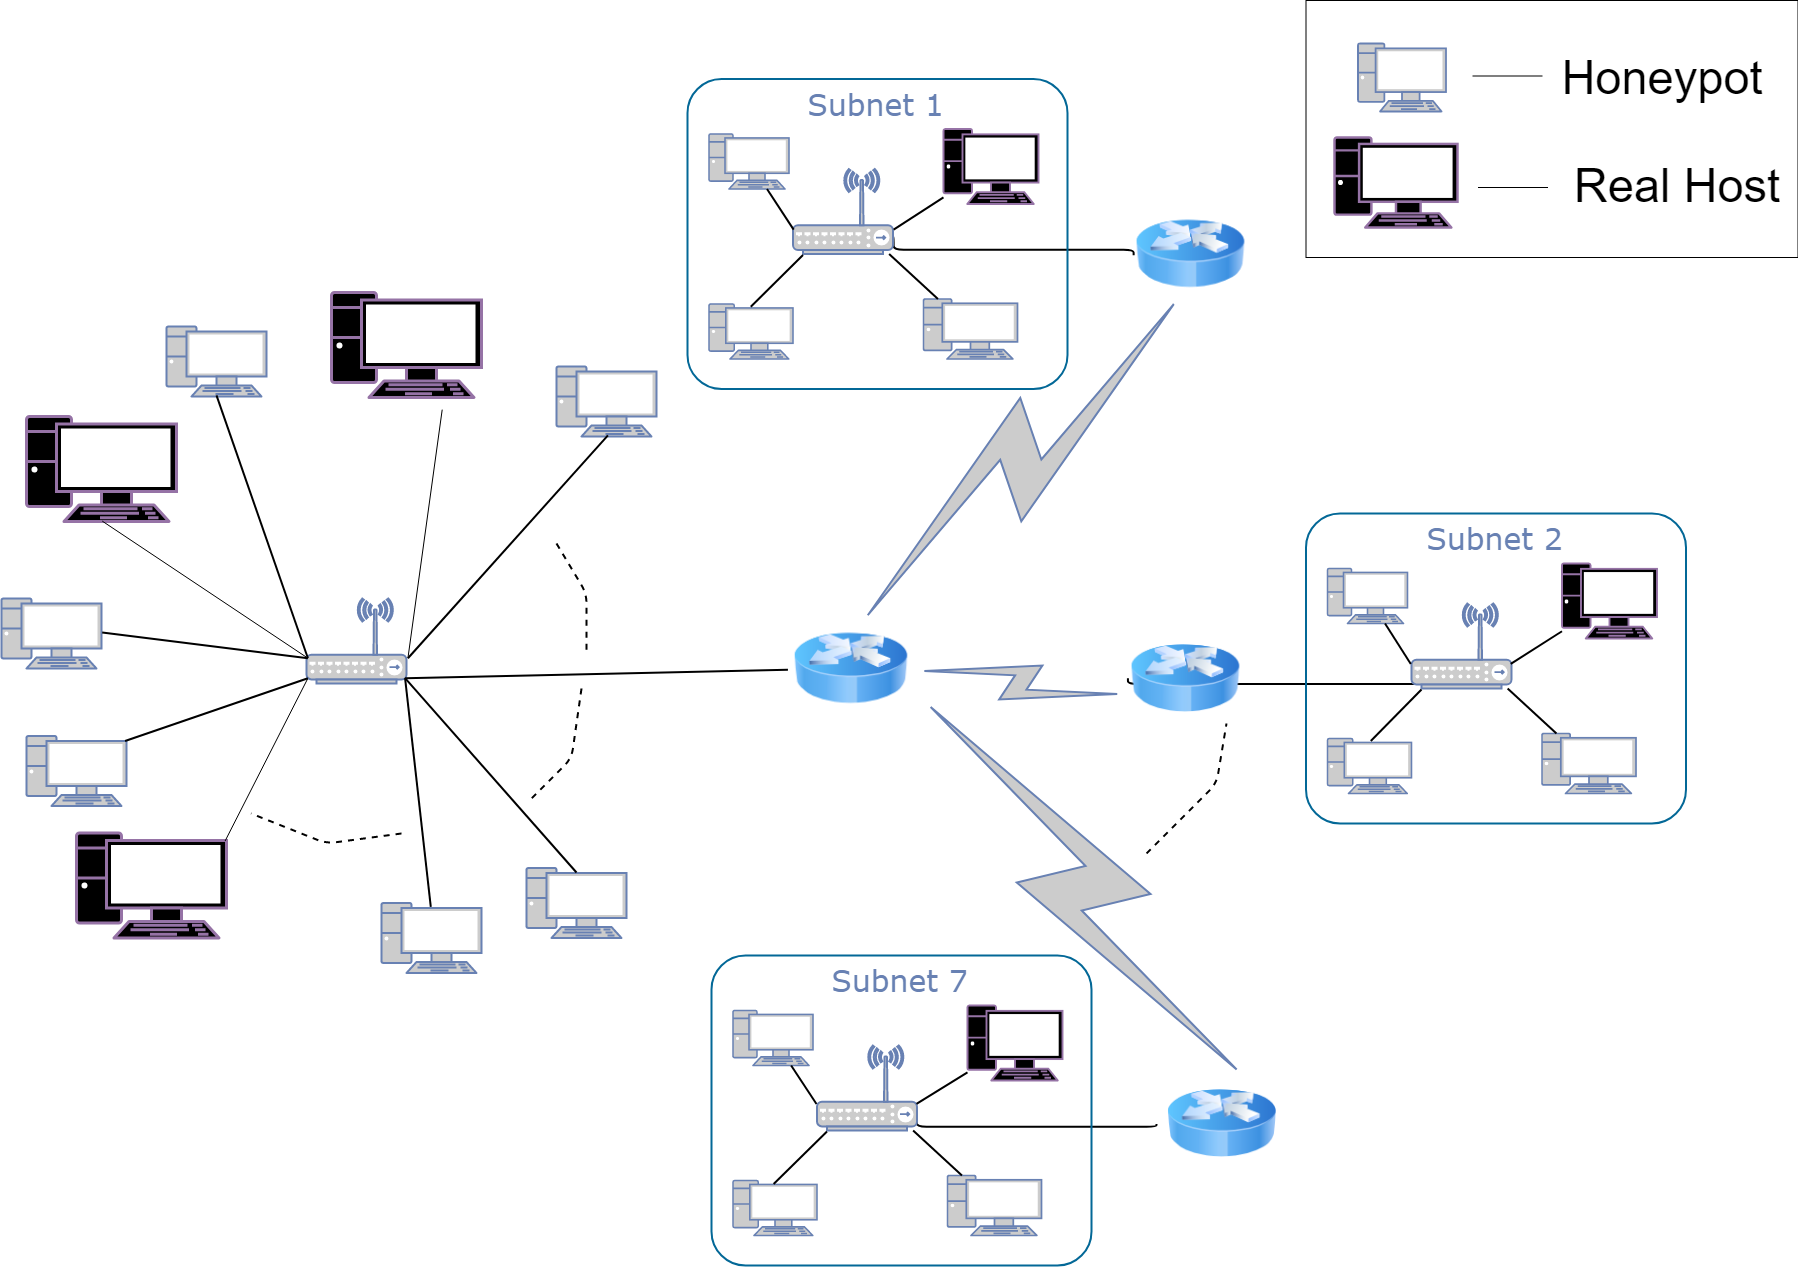
\includegraphics[scale=0.2]{Chap4/Mixed.png}
      \caption{Mixed Configuration}\label{fig:figure16}
    \end{figure} 
\section{Scanning Techniques}
So far we have learned about the various network configurations built to safeguard the network from adversaries. In this section, we would like to discuss a few reconnaissance techniques. These reconnaissance techniques can be highly effective by exploiting certain features in networks, such as the uneven distribution of hosts in the address space or the configuration of network topologies, to increase their efficiency of identifying potential targets. 
\subsection{Uniform Scanning}
Uniform Scanning probes random hosts within the scanning space and has equal chance of finding a vulnerable host \textbf{h} in a network containing \textbf{n} vulnerable hosts.
\subsection{Local Preference Scanning}
Local Preference scans IP addresses that are closer to its own local address(smaller address distance) and vulnerable hosts are detected faster by scanning the IP space where hosts are more densely distributed.
\subsection{Preference Sequential Scanning}
Preference Sequential Scanning probes the IP address space sequentially and uses local preference to select start IP address with a small address distance.
\subsection{Non-Preference Sequential Scanning}
Non-Preference Sequential Scanning selects its starting IP address in a random manner within the scanning space.It is better than preference sequential scanning (selected start IP address can be closer to addresses of vulnerable hosts).
\subsection{Preference Parallel Scanning}
Preference Parallel Scanning uses parallelism to significantly
increase the speed of scanning. It has a drawback of causing a large amount of network traffic (easy to detect). It is a simulation of a type of cooperative scanning (Group Cognition)
\section{Conclusion}
The primary goal of our system is to deceive insider adversaries, while reducing the cost to achieve increased security. In the next Chapter, we describe our experiment with human test subjects. We demonstrate that our system increases the duration required to identify vulnerable hosts in a network.

\clearpage 
